\section{The ATLAS Detector}%
\label{sec:atlas}

The ATLAS detector~\cite{PERF-2007-01}, shown in
\Cref{fig:atlas_detector_overview}, is a cylindrical particle detector
surrounding the LHC beamline at one of the IPs. The detector covers most of the
solid angle around the IP to ensure that all detectible particles from
collisions can be observed. The central part of the ATLAS detector is referred
to as the \emph{barrel}, while the two sections covering solid angles close to
the LHC beamline are referred to as the \emph{endcaps}. Going from the IP
outwards, different layers of detector technologies are used to detect and
identify different types of particles, enabling an almost full interpretation of
collision events.

\begin{figure}[htbp]
  \centering

  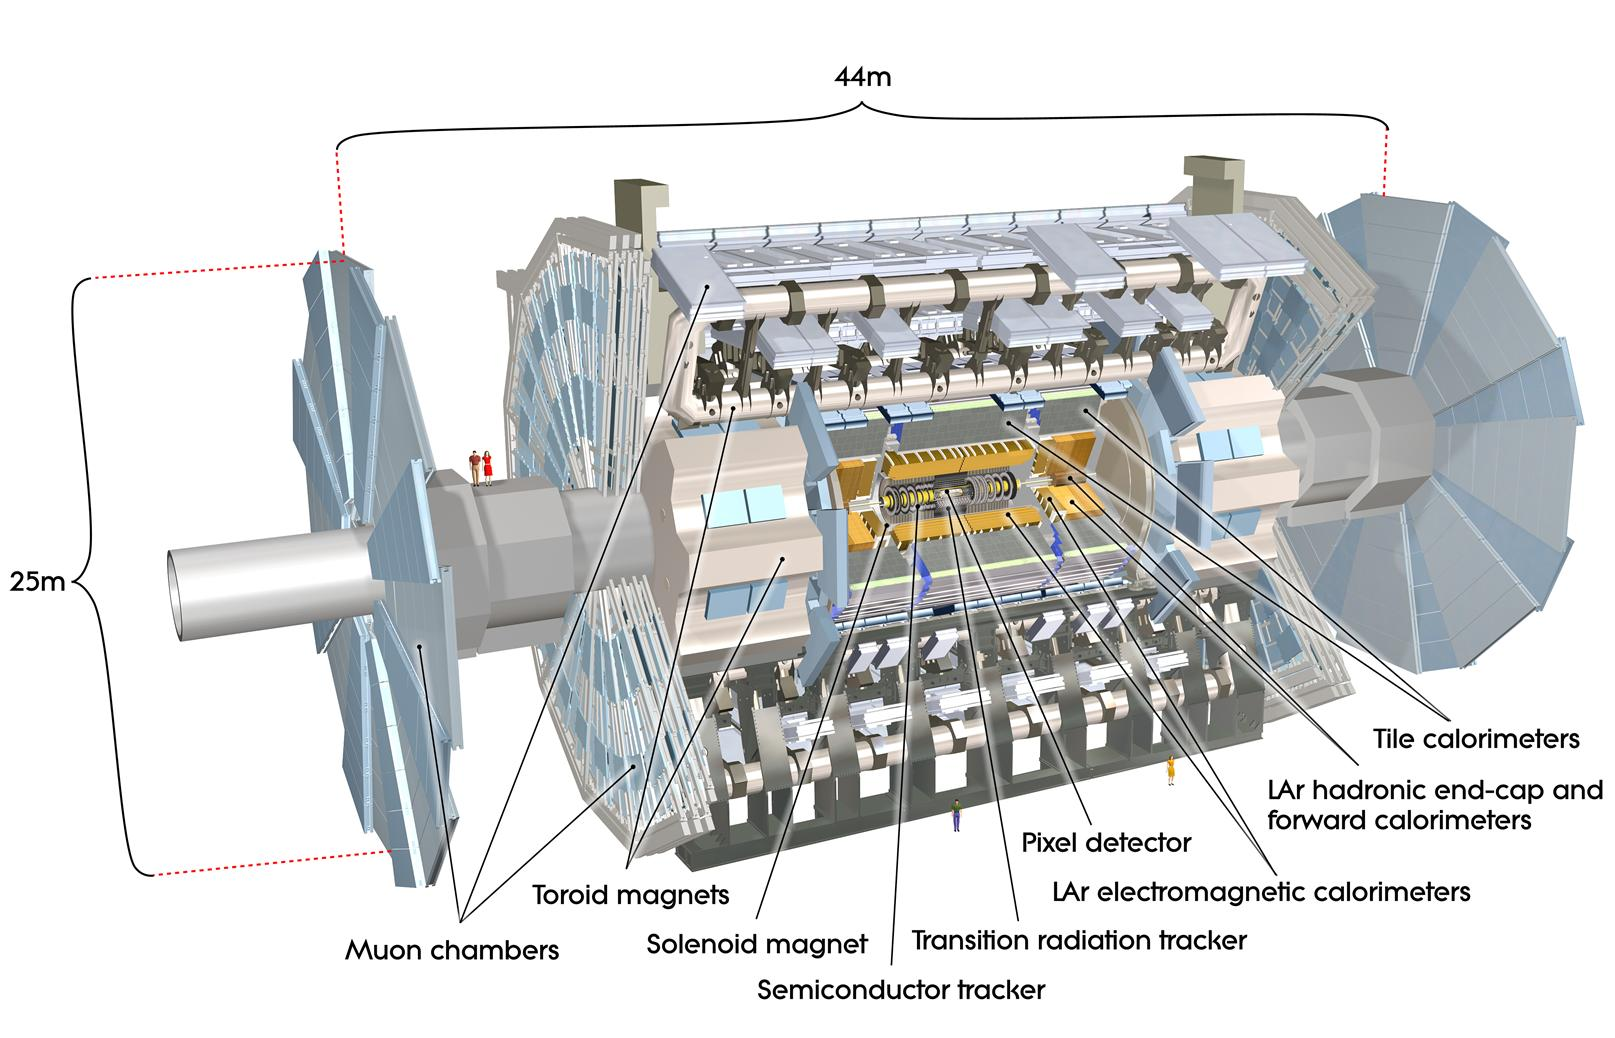
\includegraphics[width=0.76\textwidth]{atlas/atlas_overview}

  \caption{Overview of the ATLAS detector. Image taken from
    Ref.~\cite{Pequenao:1095924}.}%
  \label{fig:atlas_detector_overview}
\end{figure}

The ATLAS experiment uses a right-handed cartesian coordinate system with the
origin being located in the centre of the detector at the nominal IP. The axes
of the coordinate system are given as follows: the $x$-axis points to the centre
of the LHC, the $y$-axis points upwards, and the $z$-axis points along the LHC
beamline. The plane spanned by the $x$- and $y$-axes is referred to as the
transverse plane. A spherical coordinate system is used to specify directions in
three-dimensional space. The azimuthal angle, $\phi$, of this coordinate system
is defined as the angle in the transverse plane measured with respect to the
$x$-axis, and the polar angle, $\theta$, being the angle with respect to the
$z$-axis. With these coordinate systems, transverse momenta and energies are
defined as $\pT = \sqrt{p_x^2 + p_y^2} = p \sin\theta$ and $\ET = E \sin\theta$,
respectively. At hadron colliders, the polar angle is frequently given in terms
of the pseudorapidity \eta, which is defined as
\begin{align*}
  \eta = - \ln\tan\left( \frac{\theta}{2} \right) \,\text{.}
\end{align*}
Similarly, the angular separation between two particles is defined as
\begin{align*}
  \Delta R = \sqrt{\Delta \eta^2 + \Delta \phi^2} = \sqrt{(\eta_2 - \eta_1)^2 +
  (\phi_2 - \phi_1)^2} \,\text{,}
\end{align*}
where $\eta_1$ and $\eta_2$ are the pseudorapidities and $\phi_1$ and $\phi_2$
the azimuthal angle of both particles, respectively.

First, non-destructive measurements of electrically charged particles are
performed in the \emph{Inner Detector}, allowing to reconstruct the trajectories
of these particles.


\subsection{The Inner Detector}

\begin{figure}[htbp]

  \begin{subfigure}[b]{0.55\textwidth}
    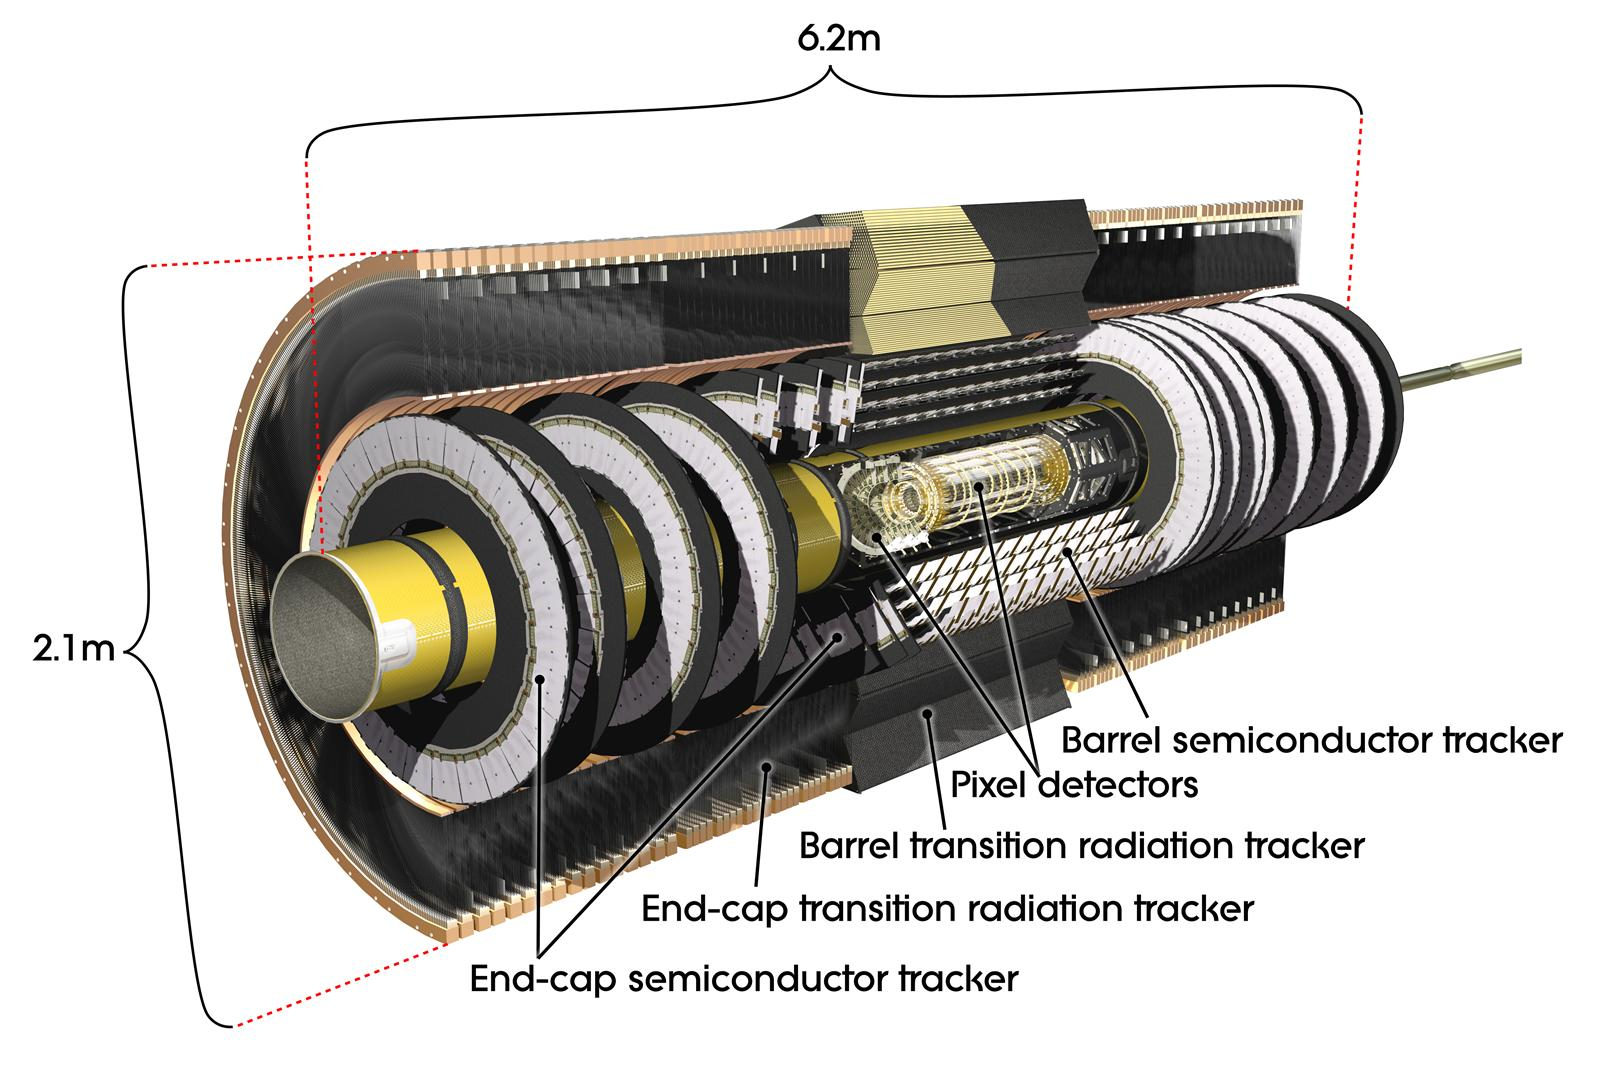
\includegraphics[width=\textwidth]{atlas/atlas_indet_1}%
    \subcaption{}
  \end{subfigure}\hfill%
  \begin{subfigure}[b]{0.45\textwidth}
    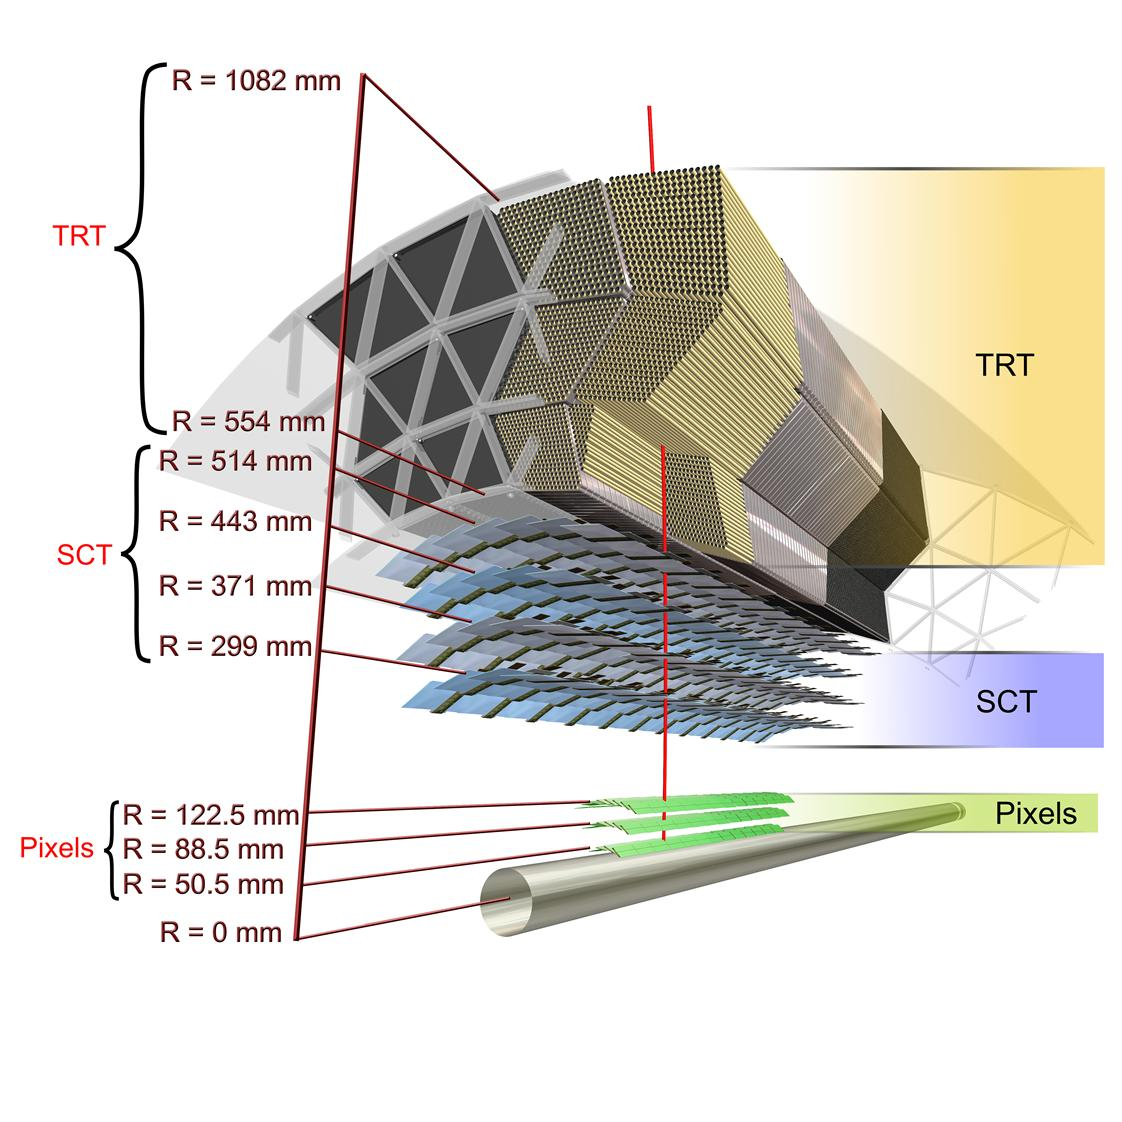
\includegraphics[width=\textwidth, trim=0 2.5cm 0 2cm]{atlas/atlas_indet_2}%
    \subcaption{}

    %[trim={5cm 0 0 0},clip]
  \end{subfigure}

  \caption{Inner detector. Images taken from
    Ref.~\cite{Pequenao:1095926}. IBL~\cite{PIX-2018-001} at
    $r = \SI{33.5}{\milli\metre}$ not displayed.}
  \label{fig:atlas_inner_detector}
\end{figure}


\subsection{Calorimeters}

\begin{figure}[htbp]
  \centering

  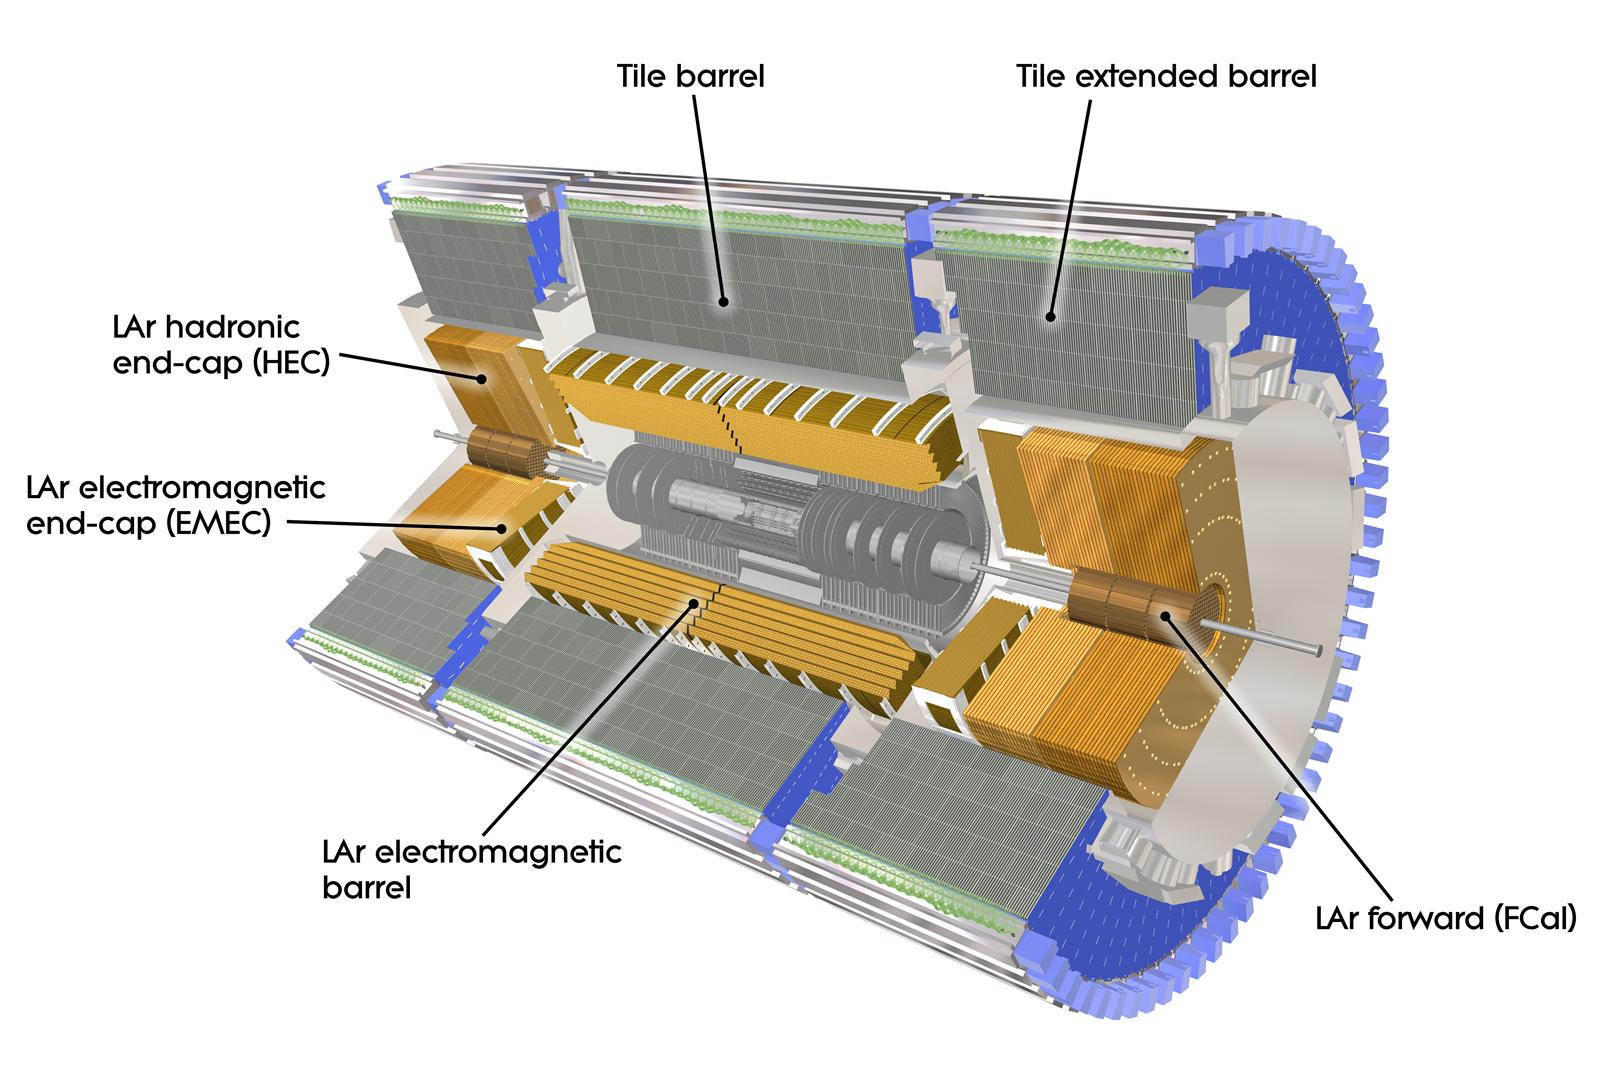
\includegraphics[width=0.65\textwidth]{atlas/atlas_calo}

  \caption{Calorimeters. Image taken from Ref.~\cite{Pequenao:1095927}.}%
  \label{fig:atlas_calorimeters}
\end{figure}


\subsection{Muon Spectrometer}

\begin{figure}[htbp]
  \centering

  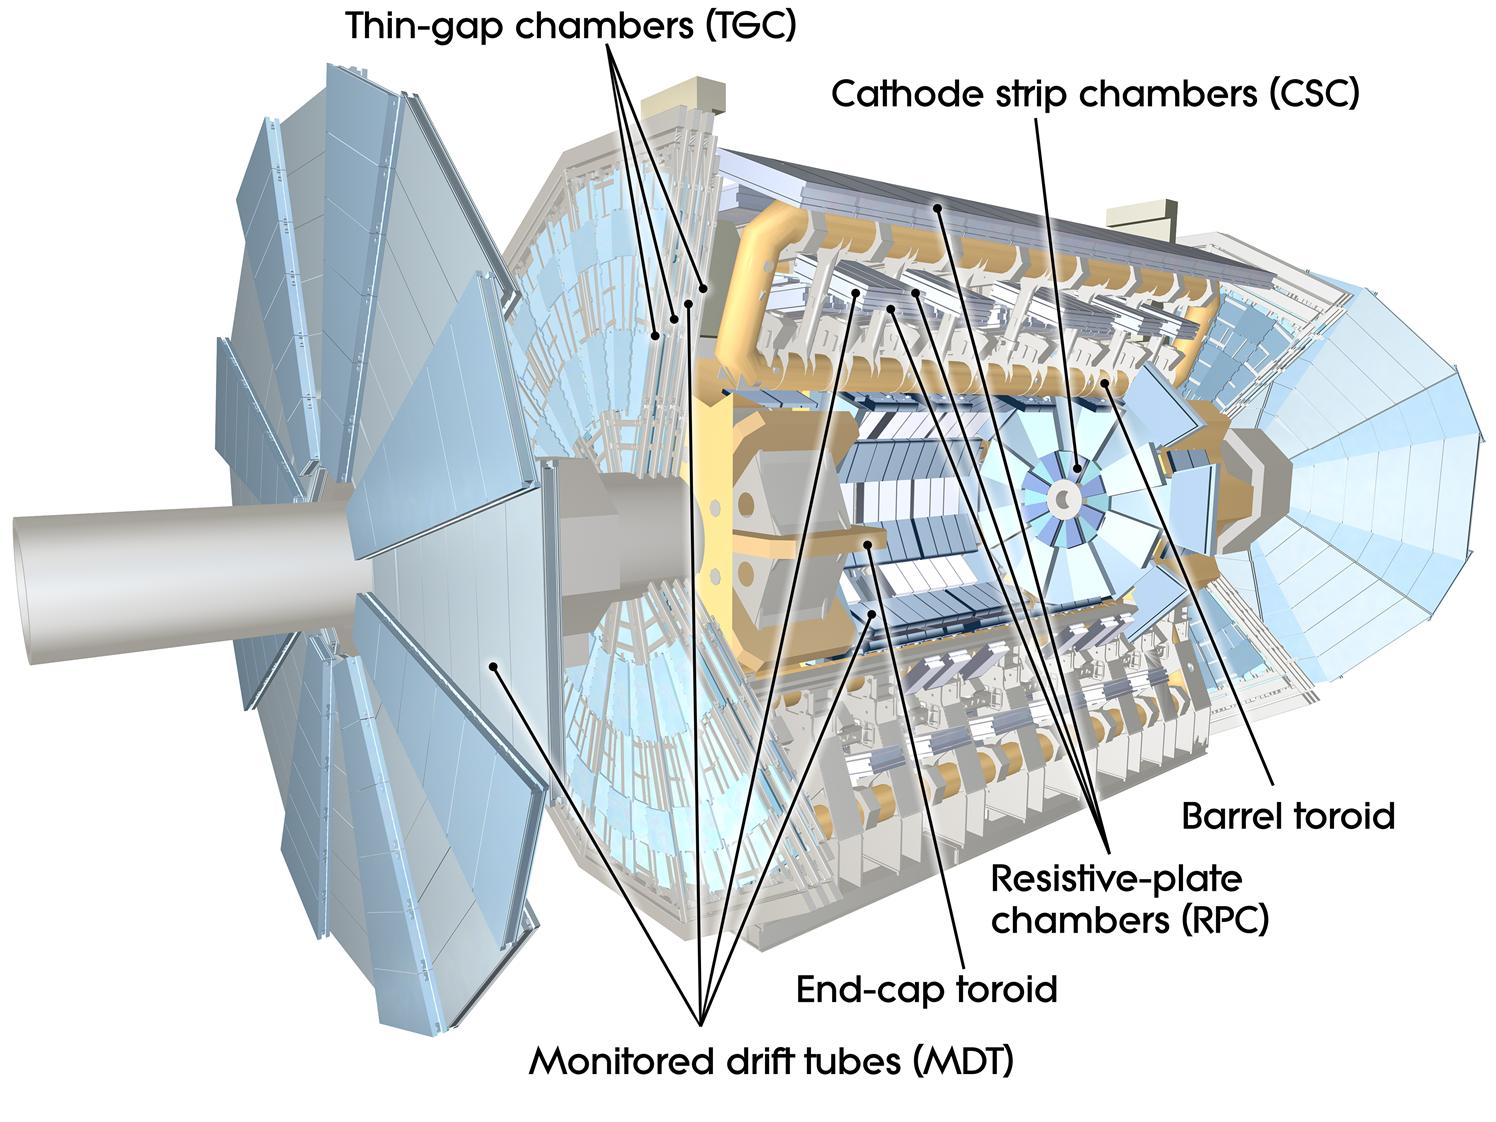
\includegraphics[width=0.65\textwidth]{atlas/atlas_muon}

  \caption{Muon subsystems. Image taken from Ref.~\cite{Pequenao:1095929}.}%
  \label{fig:atlas_muon_system}

  \todo[inline]{Is this really needed?}
\end{figure}

\subsection{Magnet System}

\subsection{The ATLAS Trigger System}

%%% Local Variables:
%%% mode: latex
%%% TeX-master: "../../phd_thesis"
%%% End:
